% Ella-Lovise  is writing

\subsection*{Problem 2.4}
\addcontentsline{toc}{subsection}{Problem 2.4}

\subsubsection*{Calculate sideslip angle}
\addcontentsline{toc}{subsubsection}{Calculate sideslip angle}

The sideslip angle is the angle from $x_b$ axis of {b} to the velocity vector of the vehicle, with positive rotation about the $z_b$ axis of {b} as given by the right-hand screw convention. The formula for sideslip is therfore:
\begin{equation}
    \boldsymbol{\beta}_r = \arcsin( \mathbf{v}^b_r/U^b_r)
    \label{eq:beta_r}
\end{equation}

defined by the relative velocity $v_r$ and relative speed $U_r$. The relative velocity in bodyframe in this assignment is defined as \eqref{eq:v_r}. The crab angle is defined in body, according to Fossen. In this assignment the relative velocity was defined to $\mathbf{v}^b_{b/n} = [1.5, 0,0]$, from problem 2.1. In problem 2.1 there was no current, and following the convention from problem 2.2, the velocity on a straight line relative to the ocean is given as $\mathbf{v}^b_{b/c} = [1.5, 0,0]$. \todo{åpen for omformuleirnger her ! } 

The sideslip angle was calculated using equation \eqref{eq:beta_r}, giving sideslip angle of $0 ^\circ$. This result is natural, since the relative velocity consists of $v=0$, since  $\mathbf{v}^b_{b/c} = [1.5, 0,0]$. Since sidelip angle is defined by the realtive velociites, and the vehicle tries to drive on a straight line, but in reality the current carries the vehicle such that the straight line becomes not as intended ( since the current is constant). \todo{Should I include plot here ? }. The result of the current carrying the vehicle will be noticeable on the crab angle, as discussed in later sections. 

\subsubsection{Simulation of translational motion of the vehicle on the circle}

The simulation of the translational motion was done by simulation in \texttt{MATLAB}. The initial conditions were : \todo{SET INN INITIAL CONDITIONS }. To simulate the translational motion without current, the velocity of the vehicle was calculated first:
\begin{equation}
    \mathbf{v}^n_{b/n} = \mathbf{R}^n_b \mathbf{v}^b_{b/c} =\mathbf{R}^n_b \mathbf{v}^b_{b/n} = \mathbf{R}^n_b [U cos(\omega t), U sin(\omega t), 0]^\top
    \label{eq:v_n_b_c}
\end{equation}

Because of no current, $\mathbf{v}^b_{b/c} = \mathbf{v}^b_{b/n}$.

The position of the vehicle was found by using Euler integration,meaning the position of vehicle is $\mathbf{p}(i+1)^n_{b/n} = \mathbf{p}(i)^n_{b/n} + \mathbf{v}(i)^n_{n}b*h $, with timestep $h = 0.1$.
 
The  simulation of the translational motion with current, was chosen to be in to ned referanceframe with the position relative to the ocean surface, meaning $\mathbf{p}^n_{b/n}$. The first step was to calculate the velocity of the vehicle $\mathbf{v}^n_{b/c}$, as done in \eqref{eq:v_n_b_c}. Furthermore the velocity of the current relative to ned, expressed in ned $\mathbf{v}^n_{c/n}$ was calculated, from equation \eqref{eq:v_n_c}. The expression for the velocity of the vehicle relative to ned reference frame, meaning  relative to the ocean surface is:


\begin{equation}
    \mathbf{v}^n_{b/n} = \mathbf{v}^n_{b/c} + \mathbf{v}^n_{c/n} =  \boldsymbol{v}^b_{b/c} + \mathbf{R}^b_n \boldsymbol{v}^{n}_{c/n} 
    \label{eq:v_b_r}
\end{equation}

The expression for the position of the vehicle relative to ned referenceframe  is found by Euler integration, meaning $\mathbf{p}(i+1)^n_{b/n} = \mathbf{p}(i)^n_{b/n} + \mathbf{v}(i)^n_{b/n}*h $, with $h = 0.1$. The method used is the same as for the simulation without current.


The crab angle, course angle and slip-angle was calculated using ??,?? and \eqref{eq:beta_r}, respectively, with $\mathbf{v}_r = \mathbf{v}^n_{b/c}$ and $\mathbf(v) = \mathbf{v}^n_{b/n}$.  Because the arcsin command in \texttt{MATLAB},\texttt{asin} only provides angles between $\frac{\pi}{2}$ and $\frac{\pi}{2}$,the crab angle and sideslip angle was approximated using $atan2(u,v)$, approximating $w= 0$.



The plots after the simulation are:

\begin{figure}[!ht]
	\centering
	\begin{subfigure}[b]{0.45\textwidth}
		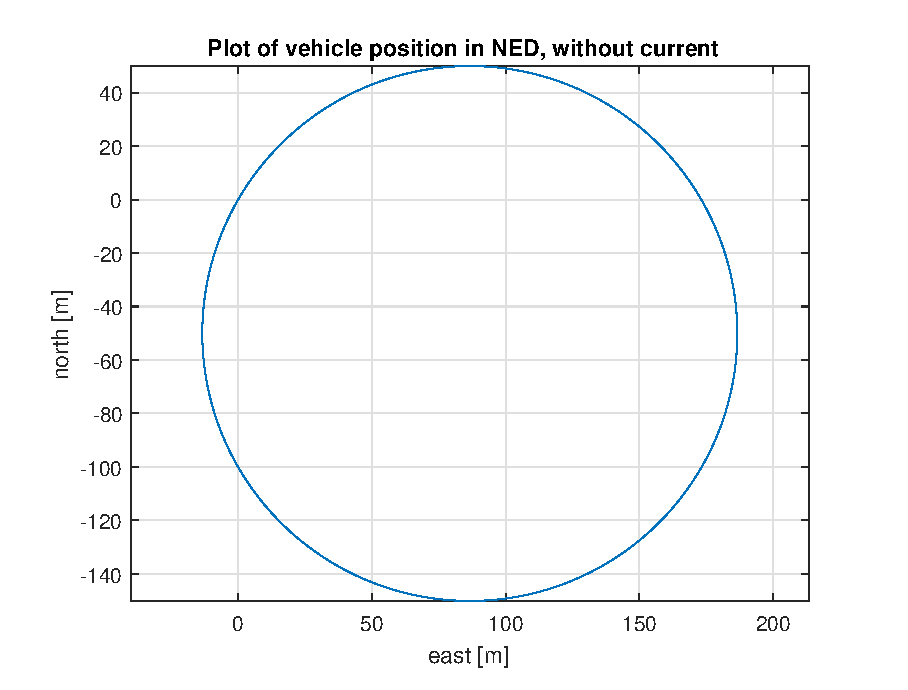
\includegraphics[width=\textwidth]{figures/4_pos.eps}
		\caption{Without current}
		%\label{fig:4_pos}
	\end{subfigure}
	~ %add desired spacing between images, e. g. ~, \quad, \qquad, \hfill etc. 
	%(or a blank line to force the subfigure onto a new line)
	\begin{subfigure}[b]{0.45\textwidth}
		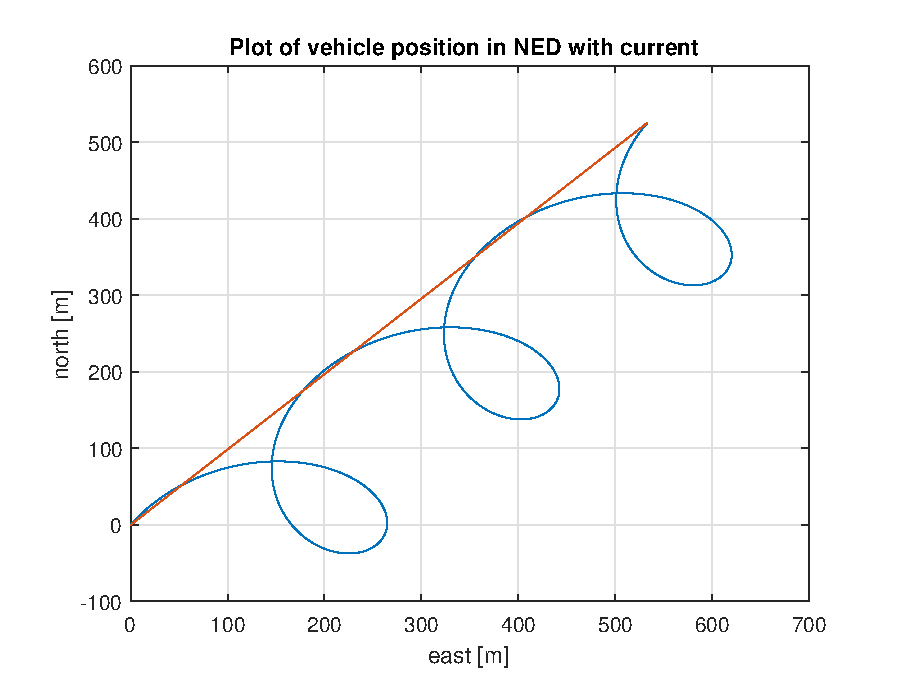
\includegraphics[width=\textwidth]{figures/4_pos_current}
		\caption{With current}
		%\label{fig:4_pos_current}
	\end{subfigure}
	\label{fig:4_pos}
	\caption{The position of the vehicle relative to ocean in reference frame ned}
\end{figure}

\begin{figure}[!ht]
	\centering
	\begin{subfigure}[b]{0.45\textwidth}
		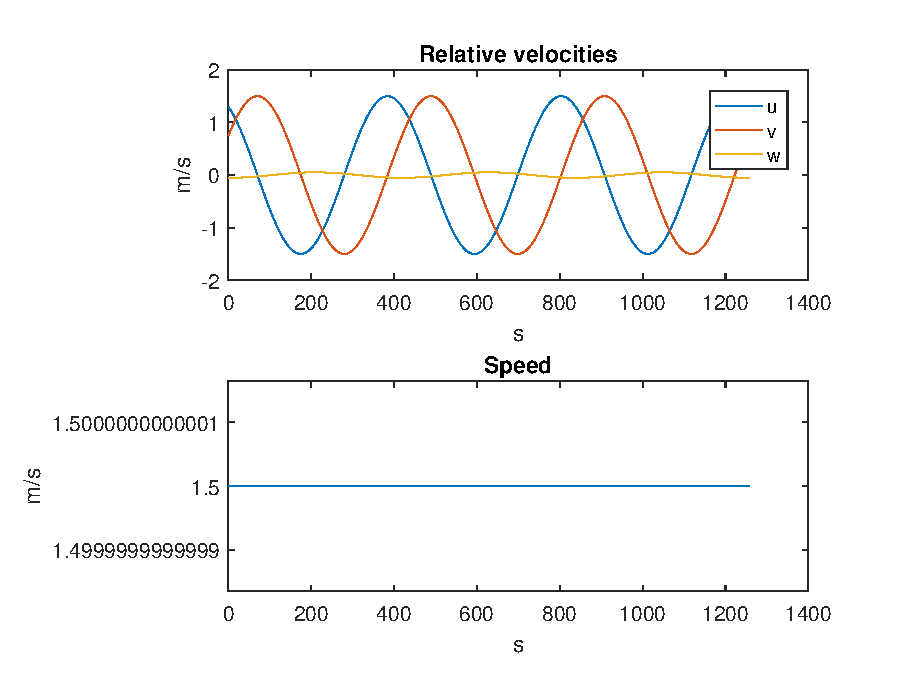
\includegraphics[width=\textwidth]{figures/4_vel}
		\caption{Without current}
		%\label{fig:4_vel}
	\end{subfigure}
	~ %add desired spacing between images, e. g. ~, \quad, \qquad, \hfill etc. 
	%(or a blank line to force the subfigure onto a new line)
	\begin{subfigure}[b]{0.45\textwidth}
		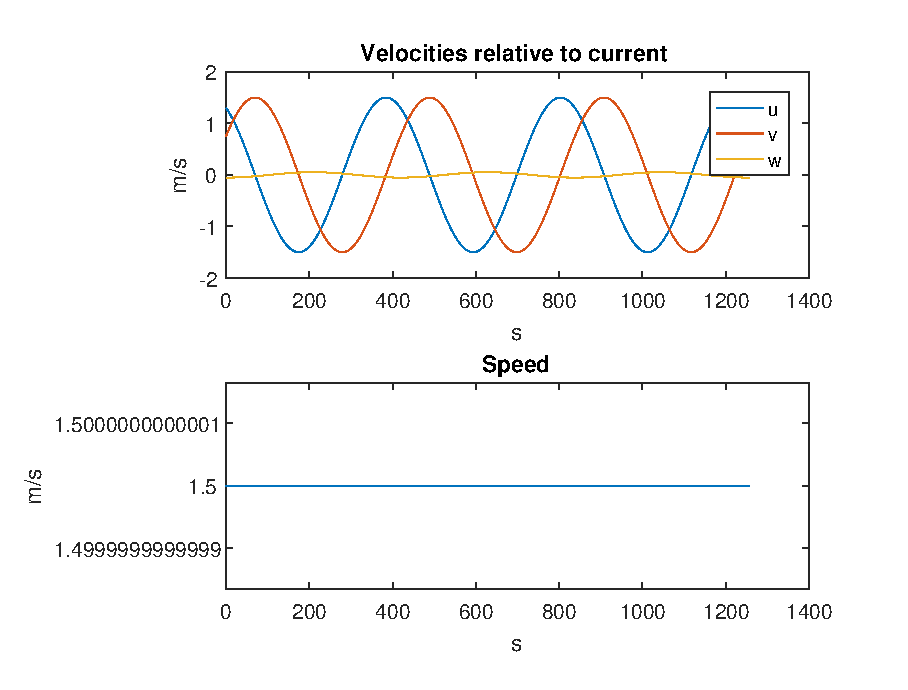
\includegraphics[width=\textwidth]{figures/4_vel_current}
		\caption{With current}
		%\label{fig:4_vel_current}
	\end{subfigure}
	\caption{The relative velocity and speed of the vehicle ,defined equation \eqref{eq:v_n_r}  in reference frame ned}
	\label{fig:4_vel}
\end{figure}

\begin{figure}[!ht]
	\centering
	\begin{subfigure}[b]{0.45\textwidth}
		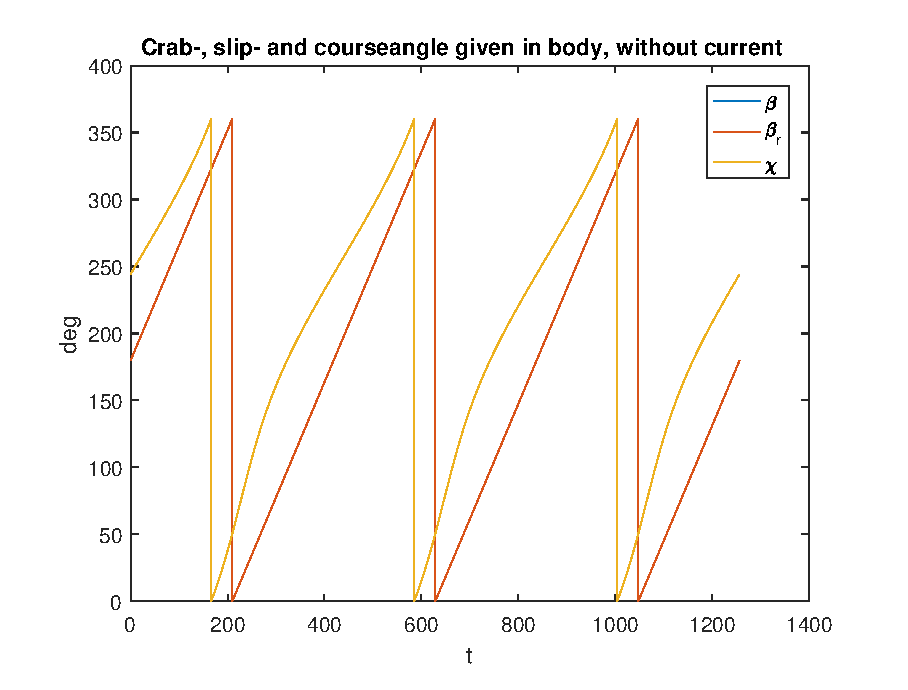
\includegraphics[width=\textwidth]{figures/4_crab_slip_course}
		\caption{Without current}
		%\label{fig:4_vel}
	\end{subfigure}
	~ %add desired spacing between images, e. g. ~, \quad, \qquad, \hfill etc. 
	%(or a blank line to force the subfigure onto a new line)
	\begin{subfigure}[b]{0.45\textwidth}
		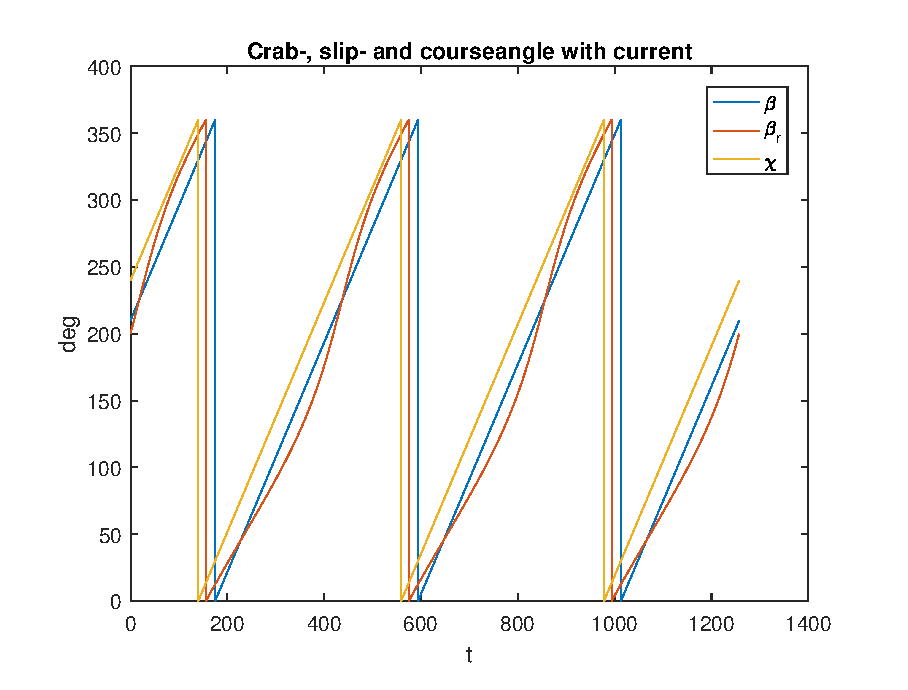
\includegraphics[width=\textwidth]{figures/4_crab_slip_course_current}
		\caption{With current}
		%\label{fig:4_vel_current}
	\end{subfigure}
	\label{fig:4_crab}
	\caption{The crab-, course and sidslipangle  in reference frame ned}
\end{figure}

In figure \figref{fig:4_pos} the position of the vehicle realtive to the ocean is plotted using referenceframe ned. Without current the vehicle makes a perfect circle with radius 100 m., as required and expected. With current the vehicle tries to make a perfect circle, but the current carries the vehicle upwards, making the path to the vehicle relative to  the ocean looking like a spiral. This is as expected, since the vehicle has velocity to drive in a circle (relative to the current), but the current carries the vehicle upstream, which makes the path of the vehicle relative to the ocean surface look as a spiral.

The speed an velocity of vehicle relative to the ocean current in NED reference frame is shown in figure \figref{fig:4_vel}. The realtive velocitites will be the same with and without current, because they we assumed that the ships velocity in body frame relative to current is $\mathbf{v}^b_{b/c} = [U \cos(\omega  *t), U \sin(\omega*t) , 0]$ and do not depend on current. Both the plots in \figref{fig:4_vel} show constant speed, since $\mathbf{v}^b_{b/c}$ consits of a cosinus and sinusoidal  depending both on the  frequency and time . The velocities as expected is periodic, with period of 1.5. \todo{check with plots}



The the velocity of the body  relative to ned , in referenceframe ned, $\mathbf{v}^n{b/n}$,  is shown in figure \figref{fig:4_vel_relative}. The speed of the vehicle realtive to ned without current is constant, same as the discussiion before since and $v^b_{b/c}=v^b_{b/n}$ and this is consistent of $[U \sin(\omega *t), U \cos(\omega*t),0]^\top$ the non rm value is $U = 1.5 m/s$. Since there is also current then, the speed and velocity of the vehicle in reference frame NED is affected by the current. Because the relative velocity is $\mathbf{v}_r = v + v_c$, and $\mathbf{v}_c != \mathbf{0}$, the speed is not constant, but varies sinusoidally. The same goes for the velocity, affected by the constant current velocities.

The plots of crab angle, slip angle and course angle goes from $0-360^\circ$. This is reasonable since the vehicle is driving in a circle with the "snout" \todo{check expression, snute på engelsk} in the same direction. In the plot without current $\mathbf{v}^b_{b/c} = \mathbf{v}^b_{b/n} $, this means $\beta_r = \beta$, and is the same result as from the plot. In the plot with current the sideslip angle $\beta_r$ are the same as in plot without current. The crabangle and course angle which depends upon the velocity of the current is therfore different in the plot with current. Since there is current both the relationship between $u^b$ and $v^b$ varies periodically, meaning the side crab angle and course angle varies periodically. The reason for this is that course angle  is linear with crab angle and yaw. \todo{should i commen't more about why goes from 0 - 360}

\subsection*{Problem 2.5}

The vehicle's turning rate is now assumed to be modeled by the Nomoto model and are:
\begin{equation}
	\frac{r}{\delta} (s) = \frac{K}{Ts+1}
\end{equation}

with $\delta$ equal the rudder angle, $K =0.1 s^{-1}$ and $T = 50s$.

The pitch and rollmotions are given as
\begin{equation}
\begin{aligned}
	&\dot{p} + 2\zeta_p\omega_p p + \omega_p^2 \phi = 0\\
	&\dot{q} + 2\zeta_q\omega_q q + \omega_q^2 \theta = 0
	\label{eq:p_q_dot}
\end{aligned}
\end{equation}
with damping factors and natural  frequencies as $\zeta_p = 0.1 $, $\zeta_q = 0.2 $, $\omega_p = 0.1 $ and $\omega_q = 0.05 $. 

\subsubsection*{Calculations of steady state}

The steady state angular velocities $p_s$, $q_s$ and $r_s$ during turning for a constant rudder angle $\delta$ may be found by setting $\dot{p}= \dot{q} = \dot{r} = 0$. The equation for $\dot{r}$ may be found by inverse Laplace using the Nomoto equation. In \cite{Fossen2011} the time representation of the first order Nomotos model, equation (7.52) in \cite{Fossen2011} is estimated as 

\begin{equation}
    T \ddot{\psi} + \dot{\psi} = K \delta
    \label{eq:nomo_first_order_time}
\end{equation}

In this problem $\theta = 2.0 ^\circ$ and $\phi = 0.0 ^\circ$, giving $\dot{\psi}$ as approximately $r$. Using \eqref{eq:nomo_first_order_time} the  first order Nomo-model time representation as:

\begin{equation}
    T \dot{r} + r = K \delta
    \label{eq:r_time}
\end{equation}

Using \eqref{eq:r_time} and \eqref{eq:p_q_dot} and setting $\dot{p} =\dot{q} = \dot{r}$ gives the following expression for the steady state of the linear velocities $\dot{\omega}^b_{b/n}$:

\begin{equation}
\begin{aligned}
	& p_s = \frac{\omega_p^2 \phi}{ 2\zeta_p\omega_p} \\
	& q_s = \frac{\omega_q^2 \theta}{2\zeta_q\omega_q} \\
	& r_s = K \delta
	\label{eq:p_q_dot}
\end{aligned}
\end{equation}

Using $\theta = 2.0$, $\phi = 0$ gives the steady-state velocities $p_s = 0$, $q_s = 0.1 ^\circ$, $r_s = 0.1 \delta$. This means that in steady state, there is approximately no angular velocities around $x_b$ and $y_b$, while around $z_b$ there is a constant angular velocity, meaning the vehicle will turn in a circle about $z_b$ as long as there is rudder. \todo{Alexandra, anything to add ?}

\subsection*{Problem 2.6}

In this problem the model of the vehicle is implemented with varying $\boldsymbol{\omega}^b_{b/n}$, described in equation \eqref{eq:r_time} and \eqref{eq:p_q_dot}. The system have the initial positions $\boldsymbol{\Theta} = [-1.0^\circ, 2,0^\circ, 0.0^\circ]^\top$ and $\boldsymbol{\omega}^b_{b/n} = [0,0,0]^\top s^{-1}$ . The start position $\mathbf{p}^n_{b/n} = [0,0,0]^\top m$. The vehicle is still exposed to the current descirbed in equation \eqref{eq:v_n_c}  and the rudder changes after 700 seconds from $\delta = 5^\circ$ to $\delta = 10^\circ$.

\subsection{Simulation}

The system is simulated in the file {\color{\blue} attitude4.m}. 


